\chapter{Motivation}
The seemingly unstoppable growth of global population compounded by climate change is putting an enormous pressure on the agricultural sector. As estimated by the World Resources Institutes (WRI), the number of people on our planet will reach an astounding 10 billion by 2050 (\cite{ayaz_internet--things_2019}) and, as a result, the agricultural production must double to keep up with the demand \cite{singh_machine_2016}. However, the agricultural sector is facing immense challenges due to plant diseases, pests and weed infestation and in these times, like never before, the switch to a more sustainable model seems inevitable. The main target of sustainable farming is to increase yield while reducing reliance on herbicides and pesticides, and therefore trying to target treatments only to plants that specifically require it by monitoring key indicators of each individual crop, a technique usually referred to as ''precision farming''. This technique is notoriously time and energy consuming, if done manually, and therefore usually discarded in favour of more traditional methodologies \cite{lottes_effective_2016}.\\
In the last years there has been, however, an increased focus on integrating cutting-edge technology with precision farming to improve quality and quantity of agricultural production, while at the same time lowering the inputs - like manual labour - significantly \cite{islam_review_2021}.  This system is also known as ''smart farming'' and it is based on the adoption of autonomous robots, which could be both wheeled robots and Unmanned Aerial Vehicles (UAVs), and it has been enabled by the astonishing advancements in the field of the Internet of Things (IoT). \\
IoT is the key technology behind smart farming and allows to add value to the data collected by automated processes by ensuring data flow between different devices  \cite{islam_review_2021}.  More importantly, IoT allows more cost-efficient and timely production and management practices, as showed by  Glaroudis et al. in \cite{glaroudis_survey_2020}, and at the same time, the reduction of the inherent climate impact by enabling real-time reactions to infestations,  such as weed, pest or diseases, and by enabling a more adequate use of resources such as water, pesticides or agro-chemicals \cite{islam_review_2021}.
In other words, IoT makes precision farming not only more efficient in terms of both money and resources, but even more sustainable than other traditional farming methods. \\
One of the cultivations which will benefit immensely by the adoption of smart farming is the sugar beet. The \textit{Beta vulgaris L},depicted in Fig. \ref{fig:sugar_beet}, commonly referred to as sugar beet, is ranked as the second most cultivated  sugar crop all over the world next to sugarcane \cite{bhadra_weed_2020}. As showed by May in \cite{may_economic_2003}, being a slow-growing crop early in the season \cite{bhadra_weed_2020}, this plant seems to be a very poor competitor against weed, a claim also backed up by Schweizer's researches, which reports that sugar beet root yields can be reduced by 26–100\% by uncontrolled weed growth.  \cite{schweizer_weed_1989}\\
\begin{figure}[ht]
	\centering
	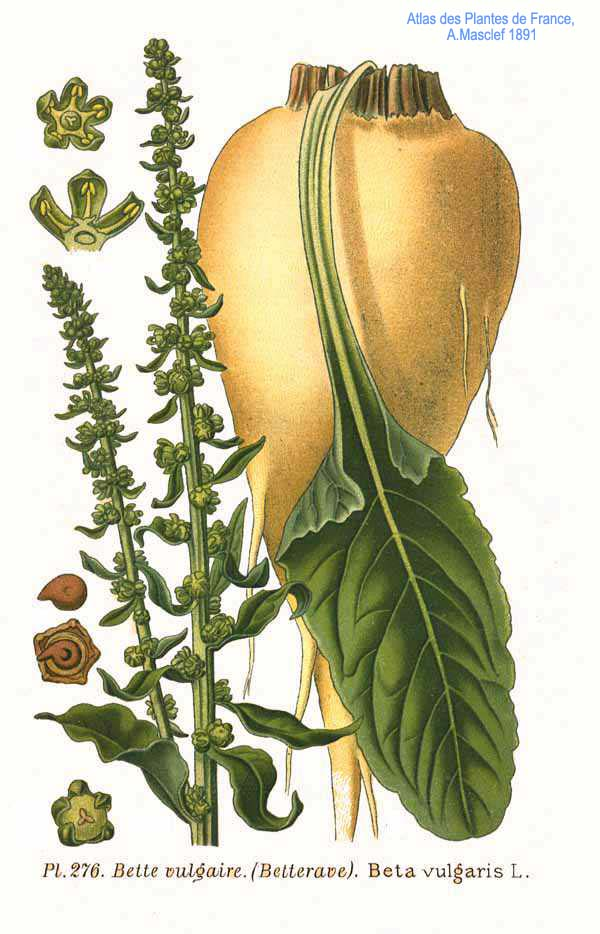
\includegraphics[width = 5cm]{img/276_Beta_vulgaris_L.jpg}
	\caption[Depiction of a sugar beet plant]{Depiction of a sugar beet plant \cite{masclef_sugar_1891} }{\centering}
	\label{fig:sugar_beet}
\end{figure}
\section{Smart Farming in Sugar Beet Plantations}
An approach based on smart farming could reduce the effect of weed infestations on sugar beet plantations and  increment the yield and the sustainability of said plantation.\\
As a matter of fact, even though tractors and hand labour are still vastly used for weed management, since the 50s herbicides have been the most used method of weed management in sugar beets farms (\cite{cioni_weed_2010}) and, apart from the well known environmental damage which the use herbicides leads to, another implication is the effect that they have on the sugar beet crops themselves. Most of the 'selective' herbicides have influence on sugar beet growth, with early symptoms showing on the leaves, which can, in all possibility, reduce the yield. \cite{petersen_review_2004}\\
To optimize and remove the effects of pesticides, the new frontier for weed management is to automatize the more traditional mechanical techniques (\cite{raja_real-time_2020}, \cite{frasconi_design_2014}, \cite{machleb_sensor-based_2021}).\\
Mechanical techniques, and even techniques which use selective spraying of herbicides, however, require that the sugar beet is localized before they can be applied to avoid ruining the plantation. In the research field, a lot of proposed solutions employ Convolutional Neural Networks (CNNs) for recognition tasks (\cite{gao_deep_2020}, \cite{suh_transfer_2018}, \cite{ramirez_deep_2020},  \cite{milioto2017real}, \cite{agriculture11111111}).\\
CNNs, however, impose great challenges to the developers. For example, in real time applications, classification time is of the highest importance since it affects the ability to respect deadlines. Furthermore, the performance of CNNs is influenced by many factors, like for e.g. training time or the data-set used for training.\\ %Table \ref{tab:models_ex_comp} shows an example of different architectures trained to recognize weed in a sugar beet plantations and how their performances can vary. \\ 
Being able to predict the performances of CNNs before their deployment will allow engineers to precisely model the application to tailor them for the CNN of their choice. \\
In this paper, we are going to investigate whether it is possible to make those predictions by empirically studying some of the metrics which can influence CNNs' performances and find correlations amongst them in order to be able to be precise, scalable and predictable in time. As the result of our investigation, we aim to develop a toolbox for the employment of CNNs in sugar beet recognition.

\section{Organization of the Paper}
In order to achieve the aforementioned goal, we will first analyse the main characteristics of CNNs in chapter number \ref{char_nn}. This will allow us to lay out the foundations for our further studies, since it is essential to have a proper grounding of what can influence the recognition of sugar beets.\\
Subsequently, in chapter number \ref{ana_models}, we will study how we can benchmark CNNs to obtain the measurements we need to find the correlations. Benchmarking is a notoriously convoluted task, however at the end of our study, we will be able to create a tool to measure performances and analyse CNNs in a precise and reproducible way.\\
Finally, with the help of our tool, in chapter \ref{ana_char} we will profile CNNs with fairly different architectures to identify correlations between their metrics so that we will be able to optimize the recognition of sugar beets. 
